%!TeX root=../tese.tex
%("dica" para o editor de texto: este arquivo é parte de um documento maior)
% para saber mais: https://tex.stackexchange.com/q/78101/183146

%% ------------------------------------------------------------------------- %%
\chapter{Implementação do Projeto}
\label{cap:Implementação}

Agora que foram definidas as mecânicas de jogo do ponto de vista de um jogador e
explicado que uma das intenções do projeto é facilitar o aprendizado de um 
iniciante em computação é preciso explicar melhor os detalhes da implementação
para concluir a segunda intenção do projeto que é permitir a extensão do jogo
por alguém que já conheça um pouco de programação ou esteja interessado em 
modificar o código fonte, inserindo novas funcionalidades. 

Para isso, essa seção divide a explicação dos arquivos do jogo agrupando por 
funcionalidades, assim entender o código de implementação torna-se mais simples.

\section{Inventário}

Dentro dos arquivos do jogo (diretório \textit{Phoenix Rising}) é encontrado na 
pasta \textit{GenericGameScenes} e administra os comandos disponíveis e a
movimentação deles na tela.

A seguir estão imagens com os nós que compõem a cena, os métodos do script
atrelado ao nó raiz, chamado \textit{Inventory} e as variáveis mais importantes
para entender o código.

\begin{minipage}[c]{0.5\textwidth}
    \begin{figure}[H]
        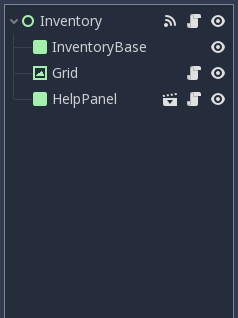
\includegraphics[scale=0.6]{../figuras/cena_inventory.png}
        \caption{Árvore da cena Inventory}
    \end{figure}
\end{minipage}%
\begin{minipage}[c]{0.5\textwidth}
    \begin{figure}[H]
        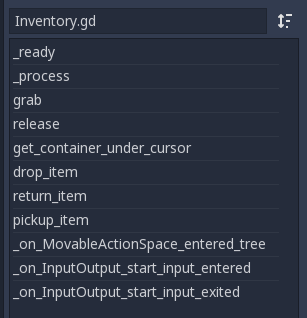
\includegraphics[scale=0.6]{../figuras/funcoes_inventory.png}
        \caption{Funções do script do nó Inventory}
    \end{figure}
\end{minipage}

\begin{figure}[H]
    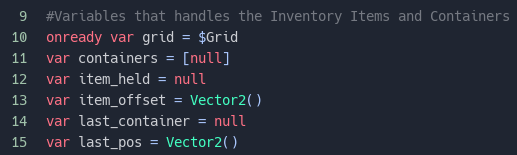
\includegraphics[scale=0.7]{../figuras/variaveis_inventory.png}
    \caption{Variáveis do script do nó Inventory}
\end{figure}

O nó \textit{InventoryBase} apenas dá cor ao espaço destinado aos comandos no
início do jogo e o nó \textit{HelpPanel} é uma cena instanciada que gerencia o
menu de ajuda que aparece ao solicitar mais explicações sobre um comando.

Dentro do jogo \textit{Phoenix Rising} os comandos disponíveis devem ocupar o
espaço de áreas específicas. Estas áreas são chamadas de recipientes (do 
inglês \textit{container}). Um recipiente pode ser o próprio \textit{Grid} do 
inventário ou espaços definidos dentro dos Espaços de Ação, que serão explicados
posteriormente.

O nó \textit{Grid} tem grande importância dentro da cena, pois é ele quem separa
cada recipiente da tela de jogo em pequenos quadradinhos, facilitando a mecânica
de mover os comandos disponíveis. Estes recipientes são adicionados na lista de 
\textit{containers}, definida na linha 11 da figura 3.3.

Para facilitar o entendimento, veja as variáveis mais importantes e o método de 
inicialização da grade (do inglês \textit{grid}):

\begin{minipage}[c]{0.5\textwidth}
    \begin{figure}[H]
        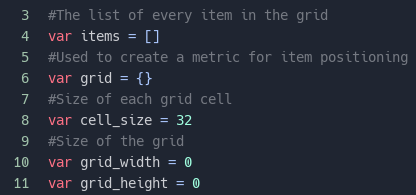
\includegraphics[scale=0.5]{../figuras/grid_variables.png}
        \caption{Variáveis do Grid}
    \end{figure}
\end{minipage}%
\begin{minipage}[c]{0.6\textwidth}
    \begin{figure}[H]
        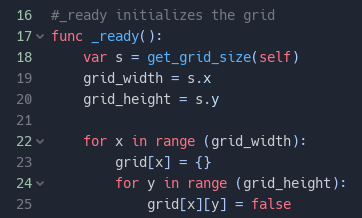
\includegraphics[scale=0.6]{../figuras/grid_ini.png}
        \caption{inicialização do Grid}
    \end{figure}
\end{minipage}

O tamanho de cada quadrado é armazenado e definido na linha 8 da figura 3.4
e as medidas da grade são armazenadas pelas variáveis definidas nas linhas
10 e 11 da mesma figura.

Na inicialização da grade do inventário o método \textit{get\_grid\_size} 
recebe o retângulo que foi definido para ser o recipiente e devolve seu 
tamanho (largura e altura) usando o sistema quadriculado, ou seja, devolve 
quantos quadrados de largura e altura ele ocupa. Depois, cada posição 
desta grade recebe o valor "falso", sinalizando que aquele quadrado está vazio,
ou seja, que nenhum item do jogo ocupa aquelas posições.

A partir dessa divisão todo comando que é disponibilizado no inventário ocupará
um número de quadrados do \textit{grid} e a movimentação destes itens é feita 
pelos métodos de pegar (do inglês \textit{grab}) e soltar (do inglês 
\textit{release}) definidos no \textit{scripts} do nó \textit{Inventory}. Ao
posicionar um comando em alguma região do recipiente os quadrados são marcados
com "verdadeiro" para sinalizar que aquela região está preenchida.

\begin{figure}[H]
    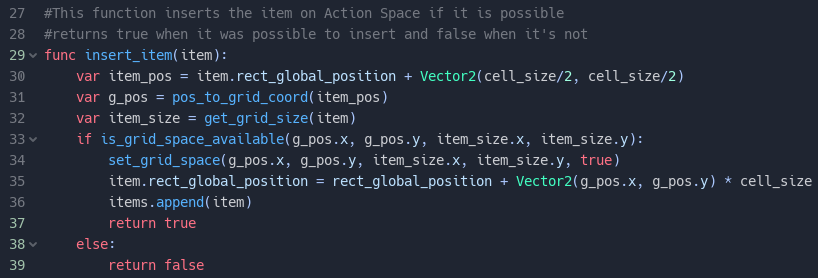
\includegraphics[scale=0.6]{../figuras/insere_item.png}
    \caption{Método de inserção de um item}
\end{figure}

\begin{figure}[H]
    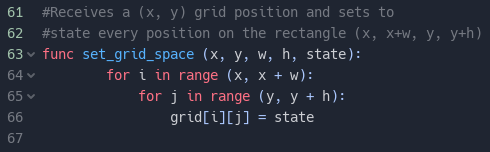
\includegraphics[scale=0.7]{../figuras/marca_grid.png}
    \caption{Marcação das posições do grid}
\end{figure}

\section{Espaço de Ação}

Dentro dos arquivos do jogo (diretório \textit{Phoenix Rising}) é encontrado na 
pasta \textit{ActionSpace}. O espaço de ação serve para conectar o sistema
fazendo com que seja possível executá-lo e posicionar os comandos que serão
utilizados no programa criado pelo jogador.

Basicamente o espaço de ação é divido em duas partes, uma móvel e outra fixa.
A cena \textit{MovableActionSpace} é a parte que permite a mobilidade e a cena
\textit{ActionSpace} cuida de receber o item posicionado e os argumentos.

\begin{minipage}[c]{0.5\textwidth}
    \begin{figure}[H]
        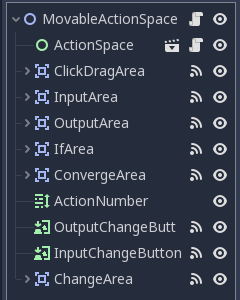
\includegraphics[scale=0.8]{../figuras/cena_movable_action_space.png}
        \caption{Cena MovableActionSpace}
    \end{figure}
\end{minipage}%
\begin{minipage}[c]{0.6\textwidth}
    \begin{figure}[H]
        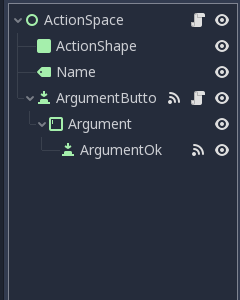
\includegraphics[scale=0.8]{../figuras/cena_action_space.png}
        \caption{Cena ActionSpace}
    \end{figure}
\end{minipage}

Note que, como \textit{MovableActionSpace} é móvel, foi utilizado um nó do tipo
Node2D e como \textit{ActionSpace} é fixo, foi utilizado um nó do tipo Control.

A cena \textit{MovableActionSpace} é formada pelos seguintes nós:

\begin{itemize}
    \item[$\bullet$]
        \textbf{\textit{ActionSpace}} - Cena que trata dos comandos e argumentos
        que são posicionados para a execução.   
    \item[$\bullet$]
        \textbf{\textit{ClickDragArea}} - Área com o ícone da mãozinha, 
        destinada a mover o espaço de ação pela tela. 
    \item[$\bullet$]
        \textbf{\textit{InputArea}} - Conexões simples de \textit{input}.
    \item[$\bullet$]
        \textbf{\textit{OutputArea}} - Conexões simples de \textit{output}.  
    \item[$\bullet$]
        \textbf{\textit{IfArea}} - Conexão complexa para administrar o comando 
        \textit{if/else}.
    \item[$\bullet$]
        \textbf{\textit{ConvergeArea}} Conexão complexa para unir os dois 
        caminhos gerados a partir de um \textit{if/else}.
    \item[$\bullet$]
        \textbf{\textit{ActionNumber}} - Indica em qual posição na ordem de 
        processamento que está aquela ação.
    \item[$\bullet$]
        \textbf{\textit{OutputChangeButton}} - Área que permite a troca da 
        conexão de saída (\textit{output})
    \item[$\bullet$]
        \textbf{\textit{InputChangeButton}} - Área que permite a troca da 
        conexão de entrada (\textit{input})
    \item[$\bullet$] 
        \textbf{\textit{ChangeArea}} - Área que marca em qual momento será feita
        a troca do valor \textit{input} definido no processo visual.
\end{itemize}

O \textit{script} atrelado ao nó \textit{MovableActionSpace} torna possível
os comportamentos descritos acima, os detalhes de como isso é feito não são
relevantes neste momento, por isso não haverá explicação detalhada sobre o 
código, entretanto os curiosos que quiserem adicionar uma nova conexão simples
de \textit{input} devem seguir os passos:

\begin{itemize}
    \item[$\bullet$]
        Seguindo o padrão de nomenclatura, criar um nó \textit{sprite} chamado
        \textit{NewConnection} e um nó 
        de forma de colisão (\textit{CollisionShape2D}) chamado 
        \textit{NewCollisionShape}, filhos de \textit{InputArea}.
    \item[$\bullet$]
        Definir a forma de colisão do nó \textit{NewCollisionShape}.
    \item[$\bullet$]
        Abrir o \textit{script MovableActionSpace.gd} e adicionar na lista
        \textit{input\_connections} o nome do nó \textit{sprite} que foi criado,
        seguindo o exemplo:
        $$\$InputArea/NewConnection$$
    \item[$\bullet$]
        Ainda no \textit{script MovableActionSpace.gd}, adicionar na lista
        \textit{input\_collisions} uma lista contendo o nome do nó 
        \textit{CollisionShape2D} que foi criado, seguindo o exemplo: 
        $$[\$InputArea/NewCollisionShape]$$
    \item[$\bullet$]
        Adicionar na lista \textit{input\_connected\_textures} o caminho que
        está a imagem referente a nova conexão quando conectada.
        O DEFAULT\_PATH está definido como "res://Accessories/art/", se a imagem
        estiver neste diretório basta adicionar:
        $$DEFAULT\_PATH + \ ''minha\_nova\_conexao.png''$$
    \item[$\bullet$]
        Adicionar na lista \textit{input\_not\_connected\_textures} o caminho
        que está a imagem referente a nova conexão quando não conectada.
        O DEFAULT\_PATH está definido como "res://Accessories/art/", se a imagem
        estiver neste diretório basta adicionar:
        $$DEFAULT\_PATH + \ ''minha\_nova\_conexao\_nao\_conectada.png''$$
    \item[$\bullet$]
        Por último basta incrementar o número total de conexões da variável
        \textit{num\_input\_connections} e pronto.
\end{itemize}

Esta sequência de ações pode ser utilizada para criar conexões de saída,
basta preencher as respectivas listas que controlam as conexões de 
\textit{output}.

O motivo das conexões serem tão importantes para este elemento do jogo vai além
de só conectar o sistema e permitir sua execução, pois cada espaço de ação 
possui também duas variáveis chamadas \textit{right\_child} 
e \textit{left\_child} que fazem referência a qual outro espaço de ação está 
conectado a sua conexão de saída, criando a árvore de execução, utilizada
pelo \textit{RunEnvironment} e \textit{VisualProcess}.

A árvore de execução permite obter a sequência de ações que o jogador projetou
no nível, além disso esta estrutura facilita o comando condicional 
(\textit{if/else}), o comando de loop e outros comandos que podem ser 
implementados como subrotinas.

Depois que o sistema está totalmente conectado, podemos criar um esquema da
árvore de execução a partir de um sistema gerador da seguinte forma:

\begin{figure}[H]
    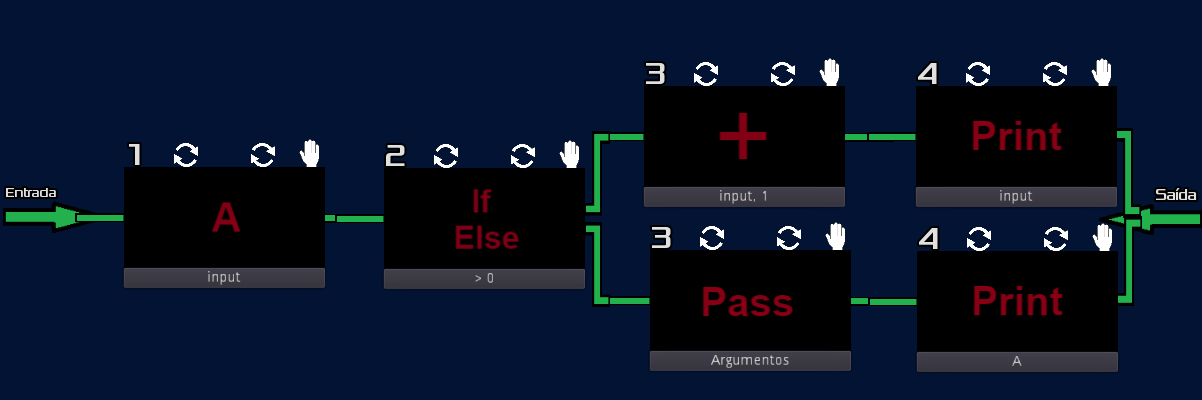
\includegraphics[width=\textwidth]{../figuras/sistema_conectado_arvore_execucao.png}
    \caption{Sistema gerador da Árvore de Execução}
\end{figure}

\begin{figure}[H]
    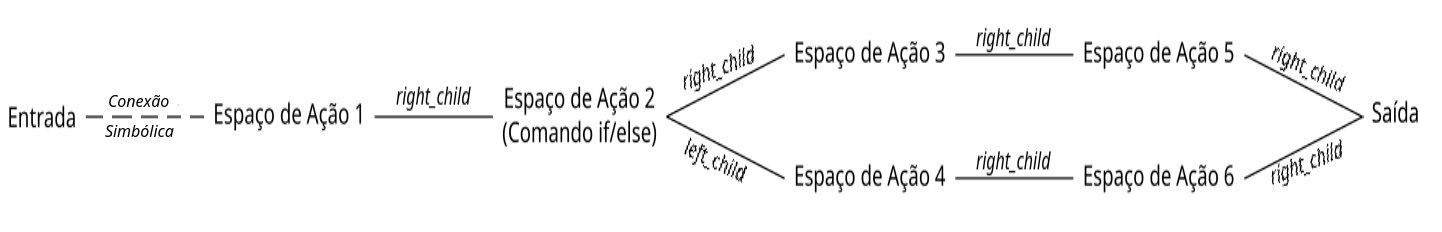
\includegraphics[width=\textwidth]{../figuras/arvore_execucao_redim.png}
    \caption{Esquema de Árvore de Execução}
\end{figure}

Vale ressaltar dois pontos importantes:

\begin{itemize}
    \item[$\bullet$]
        Os filhos da esquerda, conhecidos como \textit{left\_child}, que 
        não foram representados no esquema, para melhorar a apresentação e 
        deixá-lo mais fácil de entender, existem e possuem o valor 
        \textit{null}.
    \item[$\bullet$]
        A numeração do sistema refere-se a ordem que os comandos serão 
        executados, já a numeração do esquema enumera apenas a quantidade
        de espaços de ação que foram utilizados, portanto as numerações
        podem diferir.
\end{itemize} 

Agora será dada a exlicação sobre a cena \textit{ActionSpace}, parte fixa do 
espaço de ação mostrada na figura 3.9, que é composta pelos seguintes nós:

\begin{itemize}
    \item[$\bullet$]
        \textbf{\textit{ActionShape}} - Delimita, com um retângulo preto, o
        espaço ocupado pelo espaço de ação.  
    \item[$\bullet$]
        \textbf{\textit{Name}} - Coloca o nome "Espaço de Ação" dentro do 
        retângulo preto, pois tutorial faz referências a este item. 
    \item[$\bullet$]
        \textbf{\textit{ArgumentButton}} - Botão que permite ao jogador 
        abrir a área de preenchimento dos argumentos que serão passados para um 
        comando.
    \item[$\bullet$]
        \textbf{\textit{Argument}} - Área de preenchimento dos argumentos, 
        o que for escrito nesta área será passado como argumento para o comando
        posicionado.  
    \item[$\bullet$]
        \textbf{\textit{ArgumentOk}} - Quando pressionado fecha a área de 
        preenchimento dos argumentos.
\end{itemize}

Novamente, vale lembrar que os detalhes de implementação não são relevantes, 
basta saber que esta cena é considerada um recipiente (\textit{container}) para 
o inventário e caso um comando esteja posicionado nesta região não será possível
movimentar o \textit{MovableActionSpace} pela tela.

Uma consideração a ser feita a respeito dos argumentos serem preenchidos 
utilizando o teclado é que um menu de seleção com o mouse limitaria as opções
do jogador, sendo assim ele poderia testar todas as opções disponíveis até que 
uma delas funcionasse, indo contra o objetivo do jogo que é ensinar e não apenas 
terminá-lo. Forçar o usuário a escrever o argumento com o formato pedido faz com
que ele se acostume a ler o menu de ajuda ou as mensagens de erro e seguir os 
padrões que a computação exige, forçando-o a estar ciente do que está fazendo e
concluindo o objetivo principal que é facilitar o aprendizado.

\section{Processo Visual}

Dentro dos arquivos do jogo (diretório \textit{Phoenix Rising}) é encontrado na
pasta \textit{VisualProcess}. Este processo visual trata da animação que auxilia
o jogador a entender o que está acontecendo com os valores do programa durante
a execução.

\begin{figure}[H]
    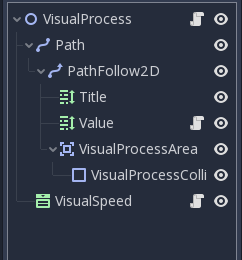
\includegraphics[scale=0.8]{../figuras/cena_visual_process.png}
    \caption{Cena Visual Process}
\end{figure}

\begin{itemize}
    \item[$\bullet$]
        \textbf{\textit{Path}} - Nó que contém a curva de pontos a ser seguida 
        pela parte visual que aparece na tela.
    \item[$\bullet$]
        \textbf{\textit{PathFollow2D}} - Trata dos pontos da curva a ser 
        seguida.
    \item[$\bullet$]
        \textbf{\textit{Title}} - Texto de identificação de qual variável a 
        parte visual está mostrando na tela. (neste projeto apenas é mostrado 
        o valor do \textit{Input})
    \item[$\bullet$]
        \textbf{\textit{Value}} - Valor corrente da variável mostrada pelo
        processo visual que é identificada pelo \textit{Title}.
    \item[$\bullet$]
        \textbf{\textit{VisualProcessArea}} - Área definida para se efetuar a
        mudança dos valores em \textit{Value}, administra alguns parâmetros da
        colisão.
    \item[$\bullet$]
        \textbf{\textit{VisualProcessCollision}} - Área de colisão (utilizada
        pela \textit{Godot}) definida para identificar o momento de se efetuar 
        a mudança dos valores em \textit{Value}.
    \item[$\bullet$]
        \textbf{\textit{VisualSpeed}} - Menu que controla a velocidade que a 
        animação do processo visual será mostrada. 
\end{itemize}

Para entender melhor o processo visual deve-se compreender o básico sobre o
funcionamento dos nós \textit{Path}
\footnote{https://docs.godotengine.org/en/3.1/classes/class\_path.html} e 
\textit{PathFollow2D}\footnote{https://docs.godotengine.org/en/3.1/classes/
class\_pathfollow.html\#class-pathfollow} na \textit{Godot}.
O nó \textit{Path} espera receber uma curva de pontos, já \textit{PathFollow2D}
pega seu \textit{Path}  pai e devolve as coordenadas de um ponto dentro dele, 
dada a distância do primeiro vértice, sendo útil para fazer outros nós seguirem 
um caminho, sem codificar o padrão de movimento. Para isso, os nós devem ser 
descendentes desse nó. Em seguida, ao  definir um deslocamento neste nó, os nós 
descendentes se moverão de acordo.

Seguindo o funcionamento de \textit{Path} e \textit{PathFollow2D} ao instanciar
\textit{Title}, \textit{Value} e \textit{VisualProcessArea} como filhos de
\textit{PathFollow2D} todos eles irão seguir o caminho da curva definida, o que
permite movimentar o valor do \textit{Input} pela tela de jogo. Veja abaixo
algumas variáveis que são utilizadas no controle deste processo:

\begin{figure}[H]
    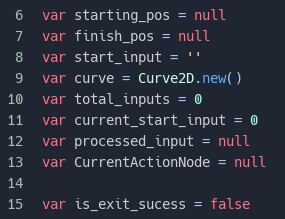
\includegraphics[scale=0.8]{../figuras/variaveis_visual_process.png}
    \caption{Variáveis Visual Process}
\end{figure}

\begin{itemize}
    \item[$\bullet$]
        \textbf{\textit{starting\_pos} e \textit{finish\_pos}} - demarcam onde o 
        processo visual inicia e onde ele termina, respectivamente.
    \item[$\bullet$]
        \textbf{\textit{start\_input}} - recebe o valor inicial da entrada.
    \item[$\bullet$]
        \textbf{\textit{curve}} - guarda a curva 
        de pontos, que será preenchida conforme a execução do programa.
    \item[$\bullet$] 
        \textbf{\textit{total\_inputs}} - guarda a quantidade de valores que foi 
        fornecido na entrada do programa
    \item[$\bullet$]
        \textbf{\textit{current\_start\_input}} - guarda qual valor da entrada que será
        processado.
    \item[$\bullet$]
        \textbf{\textit{processed\_input}} - armazena os 
        valores que se alteram durante a execução e que são exibidos na 
        animação.
    \item[$\bullet$] 
        \textbf{\textit{CurrentActionNode}} - guarda qual espaço de ação que será
        executado
    \item[$\bullet$] 
        \textbf{\textit{is\_exit\_sucess}} - sinaliza se houve algum erro 
        durante a execução.
\end{itemize}

A função que possibilita o processo visual executar as modificações no 
\textit{input} e seguir um caminho na tela é a
\textit{\_on\_MovableActionSpace\_change\_area\_entered} definida no script do
nó \textit{VisualProcess}. Esta função é chamada sempre que há colisão entre 
\textit{VisualProcessCollision} e \textit{ChangeArea}, que está definido no 
espaço de ação.

Veja abaixo o código:

\begin{figure}[H]
    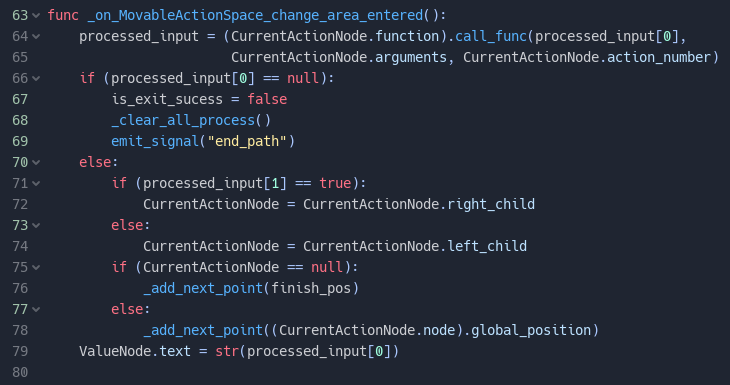
\includegraphics[scale=0.7]{../figuras/codigo_MovableActionSpace_area_entered.png}
    \caption{Variáveis Visual Process}
\end{figure}

Note que a função \textit{\_on\_MovableActionSpace\_change\_area\_entered} é 
chamada sempre que é detectada uma colisão entre um espaço de ação e o 
\textit{input}, portanto a variável \textit{CurrentActionNode} está armazenando
uma referência para o espaço de ação que colidiu.

Iniciando a função, na linha 64,
é executado o código do comando que está posicionado dentro do espaço de ação
e o novo \textit{input} que foi processado bem como qual o caminho a seguir,
serão armazenados na lista \textit{processed\_input}.

A lista \textit{processed\_input} guarda, na primeira posição (0), o valor 
resultante da operação do comando posicionado e terá \textit{null} caso algo
tenha dado errado, por exemplo um erro na passagem do argumento. O \textit{if},
na linha 66, verifica se algo deu errado na execução do comando. Caso nada
de errado tenha acontecido é executado o \textit{else}, na linha 70, que
identificará qual será o caminho que o processo visual deverá tomar.

A lista \textit{processed\_input} guarda, na segunda posição (1), qual o
caminho que deverá ser seguido, caso a posição esteja marcada com \textit{true},
então será seguido o caminho do filho da direita, se o valor for \textit{false},
então será seguido o caminho do filho da esquerda. Para entender esta parte
talvez seja necessário relembrar o que significam estes "caminhos" observando 
novamente a figura 3.11: Esquema de Árvore de Execução, definida na seção 
"Espaço de Ação".

Depois há a verificação se o processo visual chegou ao fim, na linha 75, ou 
se há mais algum ponto a seguir, na linha 77-78. Por fim, na linha 79,
atualiza-se o texto que aparece na tela para o jogador visualizar.

Note que a execução dos comandos acontece enquanto o processo visual é mostrado
na tela, assim o jogador pode acompanhar o andamento do seu programa até que
algo de arrado aconteça, facilitando o entendimento de cada comando 
individualmente e a correçao dos erros que aparecerem.

\section{Nível Base}

Dentro dos arquivos do jogo (diretório \textit{Phoenix Rising}) é encontrado na
pasta \textit{BaseLevel}

\section{Cenas Genéricas}

Dentro dos arquivos do jogo (diretório \textit{Phoenix Rising}) é encontrado na
pasta \textit{GenericGameScenes}

\section{Comportamento dos Comandos}

Dentro dos arquivos do jogo (diretório \textit{Phoenix Rising}) é encontrado na
pasta \textit{RunEnvironment}

\section{Ambiente de Execução}

Dentro dos arquivos do jogo (diretório \textit{Phoenix Rising}) é encontrado na
pasta \textit{RunEnvironment}. Este ambiente trata de construir o arcabouço 
para executar o sistema.

As imagens abaixo ilustram os nós que compõem a cena principal, chamada 
\textit{RunEnvironment.tscn} e as funções que estão definidas no script
\textit{RunEnvironment.gd} atrelado ao nó principal.

\begin{minipage}[c]{0.5\textwidth}
    \begin{figure}[H]
        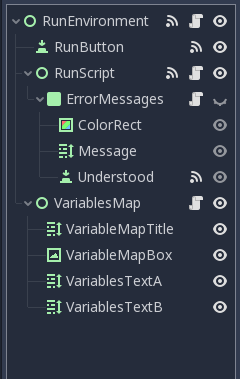
\includegraphics[scale=0.8]{../figuras/cena_RunEnvironment.png}
        \caption{Árvore da cena RunEnvironment}
    \end{figure}
\end{minipage}%
\begin{minipage}[c]{0.5\textwidth}
    \begin{figure}[H]
        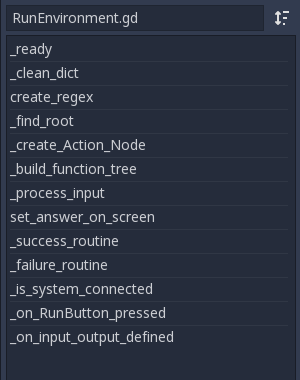
\includegraphics[scale=0.8]{../figuras/funcoes_RunEnvironment.png}
        \caption{Funções de RunEnvironment.gd}
    \end{figure}
\end{minipage}

\begin{itemize}
    \item[$\bullet$]
        \textbf{\textit{RunButton}} - Botão que, ao ser pressionado, faz com que
        inicie uma tenteativa de executar o sistema.
    \item[$\bullet$]
        \textbf{\textit{RunScript}} - Carrega o script \textit{RunScript.gd},
        neste \textit{script} estão as funções de comportamento dos comandos.
    \item[$\bullet$]
        \textbf{\textit{ErrorMessages}} - Espaço definido para a mensagem de 
        erro.
    \item[$\bullet$] 
        \textbf{\textit{ColorRect}} - Dá cor ao espaço destinado as mensagens de 
        erro.
    \item[$\bullet$]
        \textbf{\textit{Message}} - Texto da mensagem de erro.
    \item[$\bullet$]
        \textbf{\textit{Understood}} - Botão que permite fechar a mensagem de 
        erro e dar sequência ao jogo.
    \item[$\bullet$] 
        \textbf{\textit{VariablesMap}} - Carrega o script 
        \textit{VariablesMap.gd}, neste \textit{script} estão as funções que
        dão comportamento ao mapa de variáveis.
    \item[$\bullet$] 
        \textbf{\textit{VariablesMapTitle}} - Título do mapa de variáveis.
    \item[$\bullet$]
        \textbf{\textit{VariablesMapBox}} - Textura destinada ao mapa de
        variáveis.
    \item[$\bullet$] 
        \textbf{\textit{VariablesMapTextA}} - Texto da valoração da variável A.
    \item[$\bullet$] 
        \textbf{\textit{VariablesMapTextB}} - Texto da valoração da variável B.
\end{itemize}



\begin{figure}[H]
    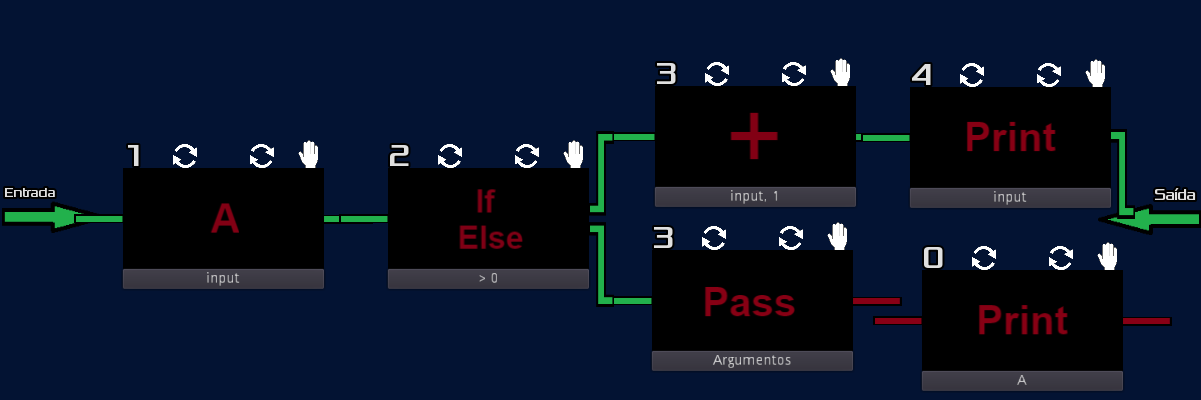
\includegraphics[width=\textwidth]{../figuras/sistema_nao_conectado_arvore_execucao.png}
    \caption{Sistema gerador da Árvore de Execução não Conectada}
\end{figure}

\begin{figure}[H]
    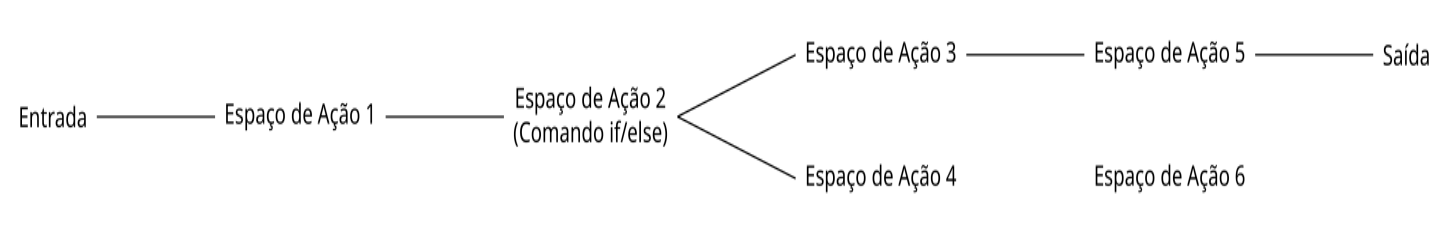
\includegraphics[width=\textwidth]{../figuras/arvore_execucao_nao_conectada.png}
    \caption{Esquema de Árvore de Execução não Conectada}
\end{figure}

\section{Ajuda ao Usuário}

Dentro dos arquivos do jogo (diretório \textit{Phoenix Rising}) é encontrado na
pastas \textit{UsersGuide} e em \textit{GenericGameScenes} 



